This section intends to discuss specific design choices that support
our multi-agent search algorithm, as detailed in our GitHub repository \cite{DiPiero2024}.
Section \ref{section_method_modeling} introduces the models and classes developed to improve our algorithm.
Section \ref{section_method_algorithm} describes the core concepts of our algorithm and provides pseudocode to guide its implementation.
Section \ref{section_method_mixed_radix} presents a mixed radix numerical representation used for the agent's path and examples to demonstrate its functionality.
Section \ref{section_method_alt_exploration_alg} presents alternative exploration strategies, including Backward Interval Filling and four Tarry algorithm variations to improve efficiency and coordination.
Section \ref{section_method_graph_visualization} highlights the algorithm's capability to handle complex graphs, as shown through an imperfect maze exploration.
Finally, Section \ref{section_method_tree_visualization} visualizes individual exploration trees for each agent, demonstrating their paths and handling of graph structures.

\section{Modeling}
\label{section_method_modeling}

In this section, we detail the modeling approach chosen to structure our problem,
emphasizing the use of classes to achieve greater flexibility in our solution.
The main classes include \textbf{Simulation}, \textbf{Graph} and \textbf{Agent}, each of which will be defined in subsequent sections.
Figure \ref{fig:class_diagram} presents a simplified class diagram that illustrates the overall structure of our model.

\begin{figure}[ht!]
    \centering
    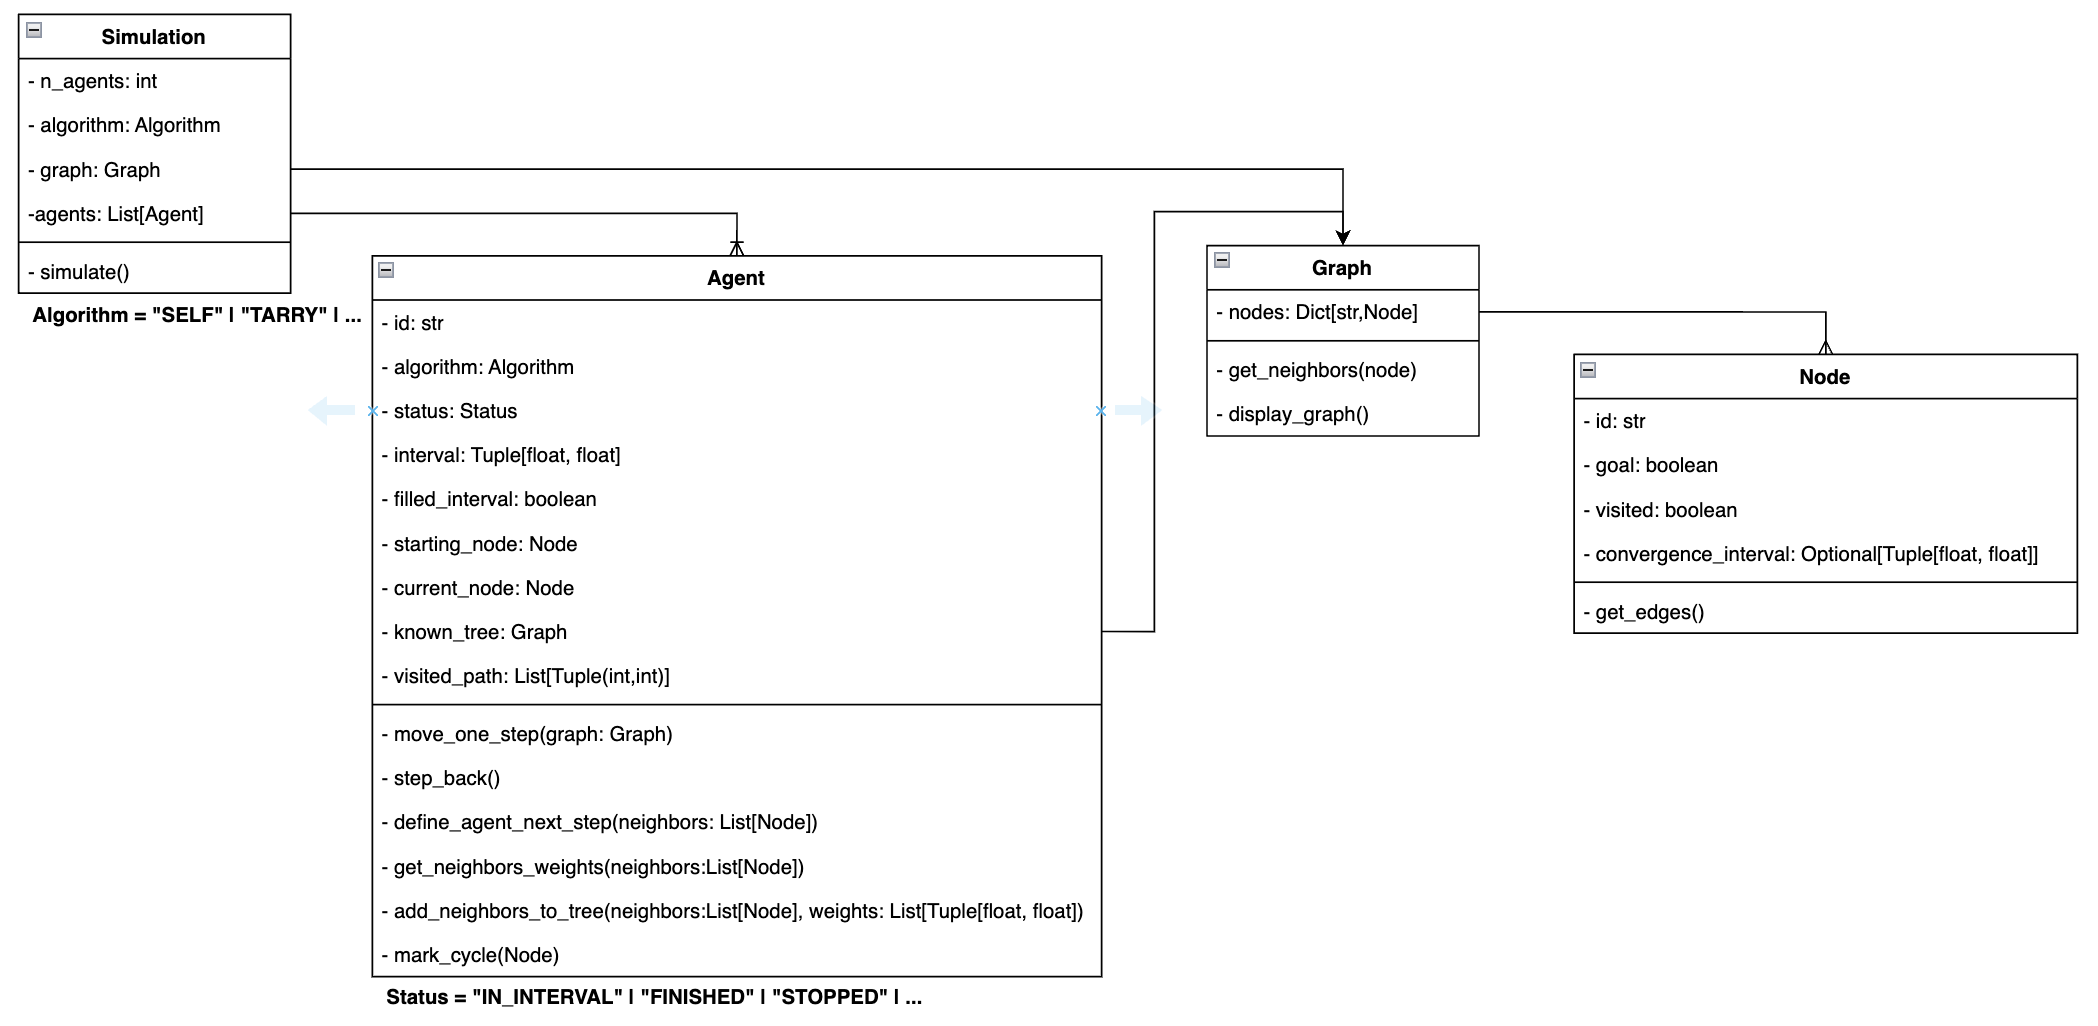
\includegraphics[width=0.9\textwidth]{Cap2/simplified_class_diagram.png}
    \caption{Simplified Class Diagram of the Multi-Agent Maze Exploration Model}
    \label{fig:class_diagram}
\end{figure}

\subsection{Simulation}
\label{section_modeling_simulation}

The \textbf{Simulation} class acts as a central controller in our multi-agent
graph exploration problem. It is primarily responsible for managing shared information, including the graph structure.
Additionally, it orchestrates the agents and the overall execution of the exploration process.

In more detail, its responsibilities include:

\begin{itemize}
    \item Shared Information: Storing and managing all information that is common between agents.
    \item Orchestration: Coordination agent activities and possible interactions during the exploration.
    \item Visualization: Providing tools for tracking the progress and visualizing the result of the exploration.
    \item Metrics: Collecting and analyzing performance metrics of the exploration.
\end{itemize}

As shown by Figure \ref{fig:class_diagram}, the core method of the \textbf{Simulation} is $simulate$ that is responsible for starting the exploration and managing each agent
in parallel, until all agents have reached the goal or have no more moves available.
The pseudocode in Algorithm \ref{alg:simulate} provides a breakdown of the function's steps and logic.

\begin{algorithm}
\caption{\textbf{Simulation} - simulate()}
\label{alg:simulate}
\begin{algorithmic}

    \State /* \textit{Graph to be explored} */
    \State graph $\gets$ $Graph()$

    \State /* \textit{Agents} */
    \State agents $\gets$ $[Agent(0), Agent(1), Agent(2), ...]$
    \State

    \State /* \textit{Agents that stopped already} */
    \State agents\_stopped $\gets$ $[$ $ ]$
    \ForAll{agent in agents}
        \State append(agents\_stopped, FALSE)
    \EndFor
    \State

    \State /* \textit{Exploration} */
    \While{False in agents\_stopped}
        \ForAll{agent in agents}
            \State /* \textit{Moving each agent in parallel} */
            \State agent.move\_one\_step()
            \If{agent.status == "FINISHED" or agent.status == "STOPPED"}
                \State agents\_stopped[agent.id] $\gets$ TRUE
            \EndIf
        \EndFor
    \EndWhile
    \State 
    \State /* \textit{Calculating Metrics} */
    \ForAll{agent in agents}
        \State /* \textit{Simplified function for calculating metrics} */
        \State calculate\_metrics(agent)
    \EndFor
    \State
    \State /* \textit{Simulation is complete} */
    \State /* \textit{Showing graphical result} */
    \State /* \textit{Simplified function for displaying} */
    \State display\_demo\_exploration(agents)
\end{algorithmic}
\end{algorithm}
    

\subsection{Graph}
\label{section_modeling_graph}

The \textbf{Graph} class, as introduced in Section \ref{section_definitions_graph},
serves as a basic representation of the graph structure for our multi-agent exploration.
Our implementation is built over the graph library NetworkX \cite{Hagberg2008}, allowing for the efficient management of nodes and edges and facilitating the agents' traversal of the graph.


A key method within this class is $get\_neighbors$.
This method returns a list of neighboring nodes in a specific order, aiding in the consistent traversal of the graph.

\subsection{Agent}
\label{section_modeling_agent}

The \textbf{Agent} class represents an agent, as defined in Section \ref{section_definitions_agent} and illustrated in Figure \ref{fig:class_diagram}.

An \textbf{Agent} is uniquely identified by its $id$ field and possesses the $status$ and $algorithm$ fields,
which define its behavior during each step of the exploration process.

Additionally, an \textbf{Agent} records its path using its own graph, defined by the $known\_graph$ field,
and a mixed radix representation of it in the $visited\_path$ field. 

Furthermore, the \textbf{Agent} possesses the $current\_node$ field, which stores its current position in the graph, and the $interval$ field, specific to our graph exploration algorithm, aiding in its traversal strategy.

The core method of the \textbf{Agent} class is $move\_one\_step$,
which is responsible for determining the agent's next action during the exploration,
as demonstrated in Algorithm \ref{alg:simulate}.
While the detailed logic of how the agent decides on its actions will be discussed in Section \ref{section_method_algorithm},
we provide a pseudocode representation of this method in Algorithm \ref{alg:move_one_step}.


\begin{algorithm}
\caption{\textbf{Agent} - move\_one\_step()}
\label{alg:move_one_step}
\begin{algorithmic}
    \Procedure{move\_one\_step}{self, graph}:
    \State /* \textit{Checking if the agent has already stopped or finished} */
    \If{self.status == "FINISHED" or self.status == "STOPPED"}
        \State \textbf{return}
    \EndIf
    \State
    \State /* \textit{Get current position} */
    \State current\_position $\gets$ graph[self.current\_node]

    \State
    \State /* \textit{Taking new step} */
    \State /* \textit{Neighbors are returned following a specific ordering} */
    \State neighbors $\gets$ graph.get\_neighbors(current\_position)
    \State /* \textit{Get only non visited neighbors} */
    \State non\_visited\_neighbors $\gets$ $[$ $ ]$
    \ForAll{neighbor in neighbors}
        \If{self.known\_tree[neighbor].visited == FALSE}
            \State append(non\_visited\_neighbors, neighbor)
        \EndIf
    \EndFor
    \State /* \textit{This decision will be explained in Section \ref{section_method_algorithm}} */
    \State next\_step $\gets$ self.define\_agent\_next\_step(non\_visited\_neighbors)
    \State /* \textit{If invalid next\_step, just move back} */
    \If{next\_step == "-1"}
        \State self.step\_back()
        \State \textbf{return}
    \EndIf

    \State
    \State /* \textit{Updating after step} */
    \State self.current\_node $\gets$ next\_step
    \State self.known\_tree[self.current\_node].visited $\gets$ TRUE
    \State
    \State /* \textit{Checking if in goal} */
    \If{current\_position.goal == TRUE}
        \State self.status $\gets$ "FINISHED"
        \State \textbf{return}
    \EndIf

    

    \EndProcedure
\end{algorithmic}
\end{algorithm}

\section{Graph Exploration Algorithm}
\label{section_method_algorithm}
As mentioned in Section \ref{section_intro_objective},
the aim of this study is to develop an effective algorithm for graph exploration using multiple agents without communication between them.
A significant challenge in this context is avoiding the redundant exploration of nodes already visited by other agents,
as it consumes resources without contributing new information to the overall exploration.

To address this problem, we adopt the solution proposed by \citen{Arthur2023}, that consists on dividing the graph into distinct intervals,
which are then split among the agents.
This approach ensures that each agent explores a unique section of the graph,
thereby minimizing overlap and maximizing efficiency.
The intervals are determined based on the number of agents, ensuring a non-overlapping distribution of the graph's nodes.
Figure \ref{fig:graph_dispersion} illustrates this concept, showing a graph with intervals assigned to different colored agents.

\begin{figure}[ht!]
    \centering
    \begin{forest}
        for tree={
            circle,
            draw,
            minimum size=2em,
        }
        [root, label=above:{\textit{Starting point}}
            [,fill=red!100
                [,fill=red!100
                    [,fill=red!100]
                    [,fill=red!100]
                ]
                [,fill=red!100
                    [,fill=red!100]
                    [,fill=red!100]
                ]
                ]
            [,fill=blue!100
                [,fill=blue!100
                    [,fill=blue!100]
                    [,fill=blue!100]
                ]
                [,fill=blue!100
                    [,fill=blue!100]
                    [,fill=blue!100]
                ]]
            [,fill=yellow!100
                [,fill=yellow!100
                    [,fill=yellow!100]
                    [,fill=yellow!100]
                ]
                [,fill=yellow!100
                    [,fill=yellow!100]
                    [,fill=yellow!100]
                ]]]
    \end{forest}
    \caption{Three agents (Red, Blue, and Yellow) disperse from each other in a graph. Source: \citen{Arthur2023}}
    \label{fig:graph_dispersion}
\end{figure}

It is important to note that while the numerical intervals are non-overlapping,
the dispersion may not always be fair or uniform.
This is evident in Figure \ref{fig:graph_dispersion_unfair},
which illustrates three agents dispersing in an unbalanced tree,
contrasting with the more uniform dispersion shown in Figure \ref{fig:graph_dispersion}.
The graph shows the nodes colored based on the agent intervals they fall into.
If a node has more than one color, it indicates that the node is within the intervals of multiple agents.

\begin{figure}[ht!]
    \centering
    \begin{forest}
        for tree={
            circle,
            draw,
            minimum size=2em,
        }
        [root, label=above:{\textit{Starting point}}
            [,halfandhalf={red!100}{blue!100}{}
                [,halfandhalf={red!100}{blue!100}{}
                    [,fill=red!100
                    ]
                    [,fill=blue!100
                        [,fill=blue!100]
                        [,fill=blue!100]
                    ]
                    [,fill=blue!100
                        [,fill=blue!100]
                        [,fill=blue!100]
                        [,fill=blue!100, label=below:{\textit{Goal}}]
                    ]
                ]
            ]
            [,halfandhalf={blue!100}{yellow!100}{}
            ]
            ]
    \end{forest}
    \caption{Three agents (Red, Blue, and Yellow) disperse in a non-uniform graph.}
    \label{fig:graph_dispersion_unfair}
\end{figure}

Mathematically, this dispersion can be expressed by a set of equations.
Assume there are $k$ agents, denoted as $a_1,a_2,a_3,...,a_k$.
The distribution of intervals can be represented as shown in Equation \ref{eq:interval_dispersion},
based on the approach proposed by \citen{Arthur2023}.

\begin{align}
    \label{eq:interval_dispersion}
    d = 1/k \notag \\
    a_{1} \textnormal{: } [0, d[ \notag\\
    a_{2} \textnormal{: } [d, 2d[ \\
    a_{3} \textnormal{: } [2d, 3d[ \notag\\
    ...\notag\\
    a_{k} \textnormal{: } [(k-1)d, 1] \notag
\end{align}

With the division of intervals explained, we now describe the step-by-step process of our algorithm for
multi-agent graph exploration.
This algorithm extends the work of \citen{Arthur2023},
incorporating modifications to handle previously visited nodes and potential cycles.

\begin{enumerate}
    \item \textbf{Initialization}
    \begin{itemize}
        \item Each agent is assigned a unique identifier and a specific interval based on Equation \ref{eq:interval_dispersion}.
        \item Each agent begins with an empty tree representation of the graph, representing the knowledge it has accumulated during the exploration. Since each agent independently explores the graph, their trees may differ, reflecting the order in which nodes are visited.
        \item All agents start at the same node, although the specific starting node is arbitrary.
        \item The starting node is assigned the interval $[0,1]$ and is added to the agent's tree.
    \end{itemize}
    \item \textbf{Exploration Strategy}
    \begin{itemize}
        \item At each step, an agent examines the adjacent nodes that have not been previously visited by it. To maintain consistency in exploration, these nodes are sorted by their unique identifiers.
        \item The agent dynamically calculates convergence intervals for each unvisited adjacent node. The calculation method is as follows:
        \begin{itemize}

            \item \textbf{Single Child}: If there is only one child node, it inherits the convergence interval of the current node.
            
            \item \textbf{Multiple Children}: If there are multiple children, the current node's convergence interval is uniformly divided among them.
            
        \end{itemize}
        \item Each adjacent node is then added to the agent's tree along with the corresponding edge and its assigned interval. 
        \item When adding a node, called the target node, to the tree in generic graphs, a cycle may be detected if the target node has not been visited yet but already appears in the tree. In this case, the new edge would form a return edge, as identified by Tarjan's Algorithm. To prevent cycles, the previous occurrence of the target node is removed from the tree, and it is then re-added with its updated edge and interval, ensuring a valid acyclic structure for the exploration tree. In Figure \ref{fig_agent_3_tree}, an example of this situation is shown. The target node was correctly removed from the agent's tree, but for demonstration purposes, a copy of the tree was created, and the target node was re-added with a modified identifier (appending "\_0" to its ID) to illustrate the cycle occurrence. That figure is based on this modified tree, not the original agent's tree.
        \item The agent then chooses the first node whose convergence interval intersects with its own. If no such node exists or if all adjacent nodes have been visited, the current node is marked as explored, and the agent backtracks to the parent node.
    \end{itemize}
    \item \textbf{Completion Criteria}
    \begin{itemize}
        \item The agent continues the exploration process until it either finds the goal or fills its assigned interval. If the goal is not found within its interval, it must be within the interval of another agent.
        \item After finishing its interval, the agent may stop or adopt an alternative strategy to accelerate the search. The default behavior implemented is to do a depth-first search (DFS), ignoring nodes already explored in the initial attempt.
    \end{itemize}
    
\end{enumerate}


The steps described in the \textbf{Initialization} topic are implemented in the initialization procedures of the \textbf{Simulation} and \textbf{Agent} classes. The pseudocode presented in Algorithm
\ref{alg:define_agent_next_step} illustrates the $define\_agent\_next\_step$ method, which implements the step-by-step process described in the \textbf{Exploration Strategy} topic.

\begin{algorithm}
\caption{\textbf{Agent} - define\_agent\_next\_step()}
\label{alg:define_agent_next_step}
\begin{algorithmic}
    \Procedure{define\_agent\_next\_step}{self, unvisited\_neighbors}:

        \State /* \textit{Calculating the convergence intervals} */
        \State /* \textit{This will be explained in Section \ref{section_method_mixed_radix}} */
        \State intervals $\gets$ self.calculate\_neighbors\_intervals(unvisited\_neighbors)
        \State
        \State /* \textit{Checking for backtracking or cycle} */
        \ForAll{neighbor $n_{j}$ in unvisited\_neighbors}
            \If{self.known\_tree[$n_{j}$].interval}
                \If{self.current\_node in self.known\_tree[$n_{j}$].get\_edges()}
                    \State /* \textit{Backtrack} */
                    \State intervals[$n_{j}$] $\gets$ self.known\_tree[$n_{j}$].interval
                \Else
                    \State /* \textit{Cycle} */
                    \State /* \textit{The agent removes the previous node from its tree} 
                    \State /* \textit{so it doesn't cause a cycle} */
                    \State self.known\_tree.remove\_node($n_{j}$)
                \EndIf
            \EndIf
        \EndFor
        \State
        \State /* \textit{Adding neighbors to tree} */
        \State self.add\_neighbors\_to\_tree(unvisited\_neighbors, intervals)
     \algstore{alg1}
\end{algorithmic}
\end{algorithm}
\begin{algorithm}
\ContinuedFloat
\caption{\textbf{Agent} - define\_agent\_next\_step()}
\begin{algorithmic}
    \algrestore{alg1}
        \State
        \State /* \textit{Checking for intersecting intervals} */
        \State /* \textit{Is important to take notice that as the neighbors are ordered}
        \State /* \textit{And the interval of a neighbor is proportional to its position}
        \State /* \textit{As we will see in Algorithm \ref{alg:get_neighbors_intervals}, the neighbor are visited in}
        \State /* \textit{incresing order of intervals} */
        \ForAll{neighbor $n_{j}$ in unvisited\_neighbors}
            \State max\_neighbor $\gets$ intervals[$n_{j}$][1]
            \State min\_neighbor $\gets$ intervals[$n_{j}$][0]
            \State max\_agent $\gets$ self.interval[1]
            \State min\_agent $\gets$ self.interval[0]
            \State
            \If{max\_agent < min\_neighbor}
                \State 
                \State /* \textit{If the node's interval is on the right of the agent's interval, surely the}
                \State \textit{agent has finished its interval, since the nodes are in increasing order of}
                \State \textit{intervals as previously mentioned} */
                \State finished\_interval $\gets$ TRUE
                \State \textbf{break}
            \Else{ min\_agent < max\_neighbor \textbf{and} max\_agent > min\_neighbor}
                \State /* \textit{Found intersecting intervals} */
                \State \textbf{return} $n_{j}$
            \EndIf
        \EndFor
        \State
        \State /* \textit{If got here, didn't find any intersecting intervals } */
        \State /* \textit{If back on root, the agent filled its interval } */
        \If{self.current\_node == self.starting\_node}
            \State self.filled\_interval $\gets$ TRUE
        \EndIf
        \State
        \State /* \textit{Just step back if interval isn't filled} */
        \If{self.filled\_interval == FALSE}
            \State \textbf{return} "-1"
        \EndIf
        \State
        \State /* \textit{If interval is filled, change strategies} */
        \State self.status $\gets$ "DFS\_SEARCH"
        \State \textbf{return}
    \EndProcedure
\end{algorithmic}
\end{algorithm}

To better understand the proposed algorithm, Section \ref{section_appendix_step_by_step} in the Appendix provides a step-by-step example of its execution on the graph shown in Figure \ref{fig_imperfect_maze_exploration}. It explains how the trees in Figures \ref{fig_agent_1_tree}, \ref{fig_agent_2_tree}, and \ref{fig_agent_3_tree} are generated.

\section{Mixed Radix Path Representation}
\label{section_method_mixed_radix}

This section details how the mixed radix representation described in Section \ref{section_definitions_unary_mixed_radix}
is used to represent the path taken by the agent, including the decision taken in each node as used in Algorithm \ref{alg:define_agent_next_step}.

Our approach utilizes the same mixed radix representation technique as described by \citen{Arthur2023}.
This method allows an agent to record each decision made along the path without the need to retrospectively analyze previous choices.
Instead, it only requires the current node's convergence interval and its edges to make decisions, reducing computational overhead. This is based on the following logic:

\begin{itemize}
    \item The path starts at ``$0.$'', and the starting node is assigned the interval $[0,1]$.
    \item If the current node has a single child, the agent appends the unary digit $I_1$ to the path. This indicates that there is only one possible path to take from this node.
    \item If the current node has multiple children (e.g., $n$ children), the agent chooses the $i$th child and appends $(i-1)_n$ to the path. This notation denotes the specific choice among the available children, with $i$ representing the child's position in an ordered list and the subscript $n$ denotes the number of children or the length of the ordered list.
    \item When the agent needs to return to a parent node, it removes the last value appended to the mixed radix representation, effectively backtracking to the previous decision point.
\end{itemize}


To illustrate this concept, we present Figures \ref{fig_blue_agent_step_0}, \ref{fig_blue_agent_step_1}, \ref{fig_blue_agent_step_2}, and \ref{fig_blue_agent_step_3}, which depict the progression of the Blue agent from the starting node to the goal in Figure \ref{fig:graph_dispersion_unfair}. Figure \ref{fig_blue_agent_step_0} shows the agent at the starting node before taking the first step. Figures \ref{fig_blue_agent_step_1}, \ref{fig_blue_agent_step_2}, and \ref{fig_blue_agent_step_3} display the first three steps taken by the agent. Each figure explicitly details the path at that step and the intervals calculated for each child of the current node. Additionally, the mixed radix path representation between the \textit{Starting Point} and \textit{Goal} for the same exploration is provided, along with an example of how it can be converted into a numerical value to calculate the corresponding interval.

\begin{figure}[H]
    \centering
    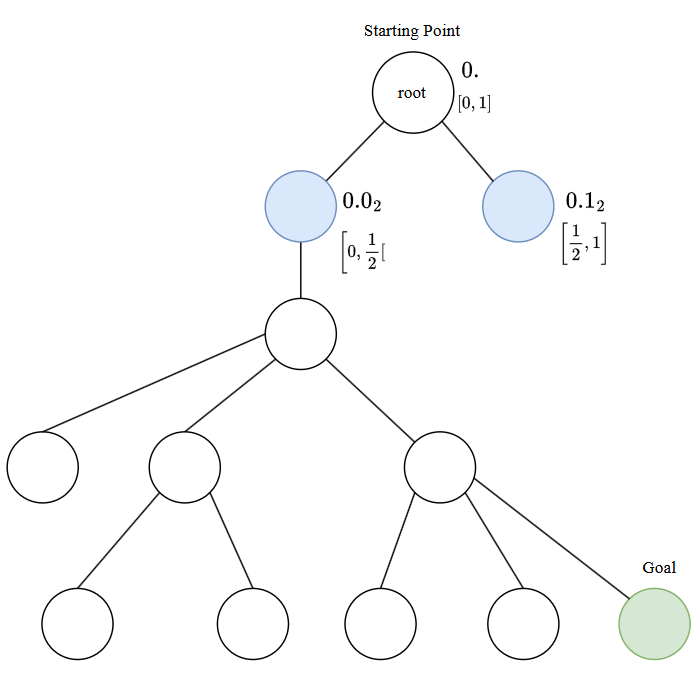
\includegraphics[width=0.6\textwidth]{Cap2/blue_agent_radix_0_step.png}
    \caption{Blue agent at the starting node of graph from Figure \ref{fig:graph_dispersion_unfair}.}
    \label{fig_blue_agent_step_0}
\end{figure}

\begin{figure}[H]
    \centering
    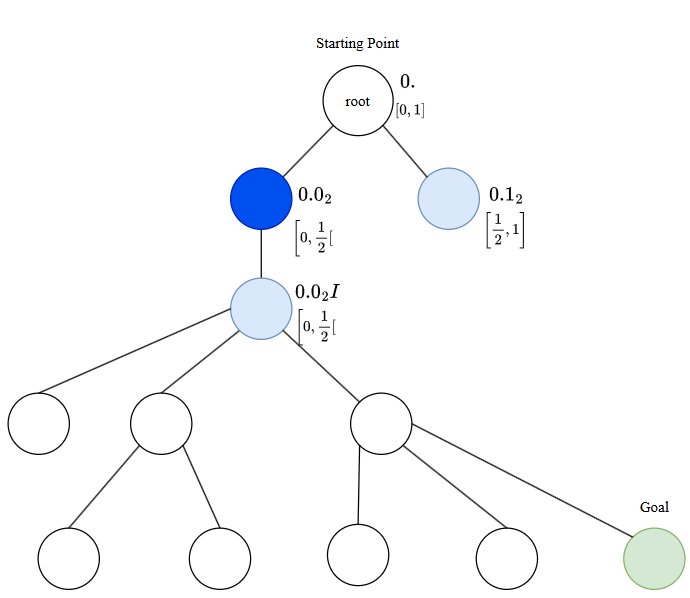
\includegraphics[width=0.6\textwidth]{Cap2/blue_agent_radix_1_step.png}
    \caption{Blue agent taking its first step in the graph from Figure \ref{fig:graph_dispersion_unfair}.}
    \label{fig_blue_agent_step_1}
\end{figure}

\begin{figure}[H]
    \centering
    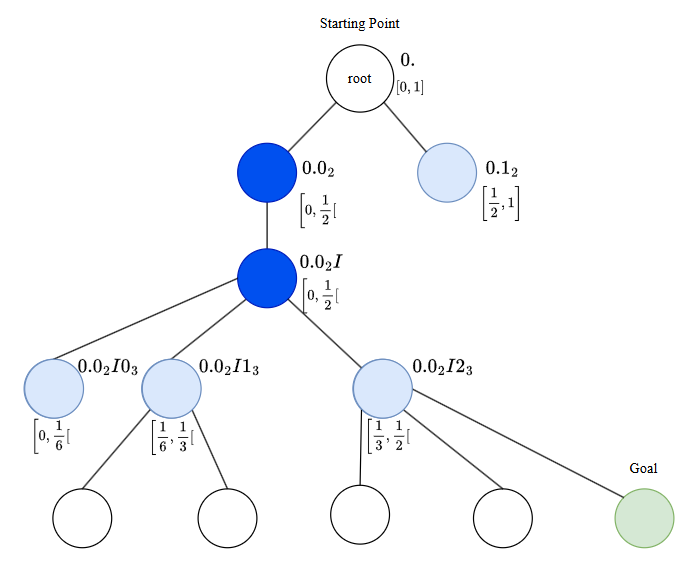
\includegraphics[width=0.6\textwidth]{Cap2/blue_agent_radix_2_step.png}
    \caption{Blue agent taking its second step in the graph from Figure \ref{fig:graph_dispersion_unfair}.}
    \label{fig_blue_agent_step_2}
\end{figure}

\begin{figure}[H]
    \centering
    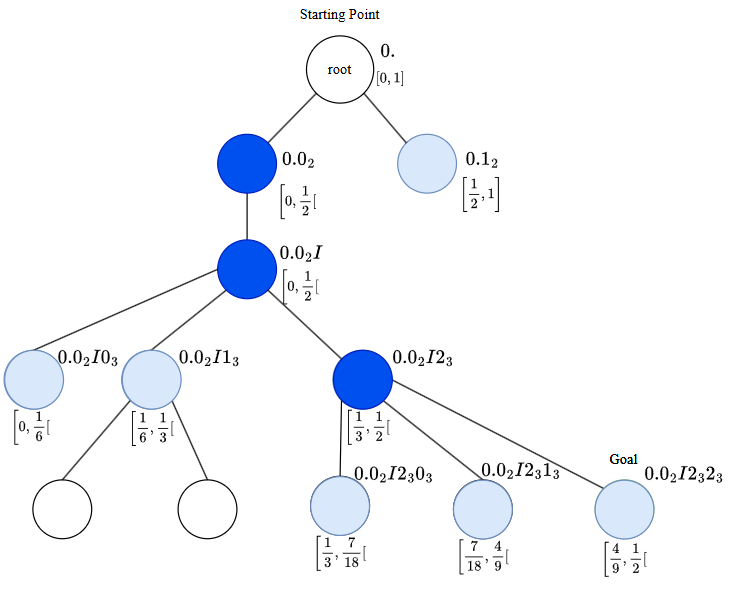
\includegraphics[width=0.6\textwidth]{Cap2/blue_agent_radix_3_step.png}
    \caption{Blue agent taking its third step in the graph from Figure \ref{fig:graph_dispersion_unfair}.}
    \label{fig_blue_agent_step_3}
\end{figure}


\begin{equation}
    x = 0_{2}I_{1}2_{3}2_{3}
\end{equation}

Following the conversion as described by Equation \ref{eq:unary_mixed_radix}, 
we can transform this mixed radix notation into a numerical value:

\begin{align}
    & x=0_{2}I_{1}2_{3}2_{3}\\
    & A=[0,I,2,2]\\
    & M=[2,1,3,3]\\
    & U=[0,2,3]\\
    & x = \sum_{k \in U} a_{k} \prod_{j=0}^{k} \frac{1}{m_j} = \dfrac{4}{9} \approx 0.4444444
\end{align}


The function $calculate\_neighbors\_intervals$ used in Algorithm \ref{alg:define_agent_next_step}
is defined by this logic and the Equation \ref{eq:unary_mixed_radix} as can be seen in Algorithm \ref{alg:get_neighbors_intervals}

\begin{algorithm}
\caption{\textbf{Agent} - calculate\_neighbors\_intervals()}
\label{alg:get_neighbors_intervals}
\begin{algorithmic}
    \Procedure{calculate\_neighbors\_intervals}{self, unvisited\_neighbors}:
    \State /* \textit{Fetching current node interval } */
    \State current\_node\_interval $\gets$ self.known\_tree[self.current\_node].interval
    \State current\_interval\_size $\gets$ (current\_node\_interval[1]-current\_node\_interval[0])
    \State interval\_chunk $\gets$ current\_interval\_size / unvisited\_neighbors.length()
    \State
    \State /* \textit{Calculating interval for each neighbor} */
    \State intervals $\gets$ $[$ $ ]$
    \ForAll{neighbor $n_{j}$ in unvisited\_neighbors}
        \State interval\_start $\gets$ current\_node\_interval[0] + interval\_chunk * $j$
        \State interval\_end $\gets$ interval\_start + interval\_chunk
        \State intervals.append((interval\_start, interval\_end))
    \EndFor
    \State \textbf{return} intervals
    \EndProcedure
\end{algorithmic}
\end{algorithm}

To ensure precision in interval calculations, we use the BigNumber library gmpy2 \cite{Martelli2015} instead of standard double-precision, which is limited to about 15 decimal places. For deeper datasets, as shown in Table \ref{tab:average_depth}, this approach is essential, as interval scales decrease by factors of $(1/2)^{depth}$. Using gmpy2 prevents rounding errors that could otherwise lead to inaccuracies in the path representation and each node's interval.

\section{Alternative Exploration Algorithms}
\label{section_method_alt_exploration_alg}

In our implementation, modifying and experimenting with variations of the exploration algorithm is simple.
By simply altering the $define\_agent\_next\_step$ function in Algorithm \ref{alg:move_one_step}, we can easily incorporate different strategies based on the agent's current status or algorithm.

In this work, we have explored six alternatives: our core algorithmm, one variation of it and four adaptations of Tarry's algorithm.

\subsection{Exploration Algorithm without Communication}
\label{section_method_zero_comm}

\subsubsection{Backward Interval Filling}
\label{section_backward_interval}

The \textbf{Backward Interval Filling} algorithm extends the primary zero-communication strategy developed in this work. Instead of initiating a new Depth-First Search (DFS) traversal after completing a designated interval, agents continue exploring by traversing the next interval in reverse order. "Next interval" refers to the interval initially assigned to the next agent in the list from Equation \ref{eq:interval_dispersion}. Note that each agent is assigned both intervals from the start, so no communication is needed. For the last agent, whose interval ends at 1, its second interval is assigned as the first agent's interval, which starts at 0. Thus, once the agent finishes exploring its original interval, it moves up on its tree to the nearest common ancestor shared with the end of the next interval, then proceeds to move downwards to the end leaf of its second interval, which it will traverse in reverse order. This variation ensures that agents remain active even after completing their primary interval, enhancing overall graph coverage and reducing idle time. It takes advantage of the fact that the tree may be unbalanced; when one interval contains significantly fewer nodes than the next, the agent assigned to the smaller interval can finish quickly and then explore the larger interval from the opposite direction. For exemplo, in Figure \ref{fig:graph_dispersion_unfair}, the yellow agent, after traversing its interval, will traverse the red nodes in reverse order.

\subsection{Exploration Strategies with Communication: Tarry Algorithm Variations}

\label{section_method_tarry_variations}

This section presents several adaptations of Tarry's algorithm that utilize communication between agents. Each variation builds upon the foundational logic of Tarry's approach but introduces different heuristics and optimizations aimed at improving performance and accommodating various graph structures.

\subsubsection{Extended Tarry Algorith}
\label{section_method_extended_tarry}

The \textbf{Extended Tarry Algorithm}, proposed by \citen{Kivelevitch2010}, is an multi-agent adaptation of Tarry's algorithm. In this approach, agents share information about visited nodes, enabling them to identify unvisited cells and determine the Last Common Location (LCL) — the most recent shared position among agents before diverging paths.The algorithm consists of two phases:

\begin{itemize}
    \item \textbf{Exploration Phase}: Each agent moves to unvisited cells, or to cells unvisited by itself, choosing arbitrarily among multiple options. If all cells have been visited, agents retreat to the last unvisited cell, marking cells as dead ends.
    \item \textbf{Cooperative Backtracking Phase}: Once an agent finds the goal and is defined as the pioneer, other agents backtrack to the Last Common Location (LCL) with it and follow the pioneer's path to the goal.
\end{itemize}

The functions $define\_next\_first\_phase\_tarry\_step$ and 

$define\_next\_second\_phase\_tarry\_step$, as shown in Algorithms \ref{alg:define_agent_next_first_phase_step} and \ref{alg:define_agent_next_second_phase_step}, implement this logic.

\begin{algorithm}
\caption{\textbf{Agent} - define\_next\_first\_phase\_tarry\_step()}
\label{alg:define_agent_next_first_phase_step}
\begin{algorithmic}
    \Procedure{define\_next\_first\_phase\_tarry\_step}{non\_visited\_neighbors}:
    \State new\_neighbors $\gets$ [] 
    \State already\_visited\_neighbors $\gets$ []
    \State /* \textit{Splitting Neighbors } */
    \ForAll{neighbor in non\_visited\_neighbors}:
        \If{neighbor not visited and not deadEnd}:
            \State new\_neighbors.append(neighbor)
        \ElsIf{neighbor visited}:
            \State already\_visited\_neighbors.append(neighbor)
        \EndIf
    \EndFor


    \If{new\_neighbors is not empty}:
        \State /* \textit{Choosing a random non-visited neighbor } */
        \State \textbf{return} random\_choice(new\_neighbors)
    \ElsIf{already\_visited\_neighbors is not empty}:
        \State /* \textit{Choosing a random non-visited by this agent neighbor } */
        \State \textbf{return} random\_choice(already\_visited\_neighbors)
    \EndIf
    \State \textbf{return} "-1" 
    \EndProcedure
\end{algorithmic}
\end{algorithm}


\begin{algorithm}
\caption{\textbf{Agent} - define\_next\_second\_phase\_tarry\_step()}
\label{alg:define_agent_next_second_phase_step}
\begin{algorithmic}
    \Procedure{define\_next\_second\_phase\_tarry\_step}{non\_visited\_neighbors,
    
pioneer\_id, pioneer\_effective\_path, lcl}            
        \If{self.status == "TARRY\_FIRST\_PHASE"}
            \State self.status $\gets$ "TARRY\_SECOND\_PHASE"
        \EndIf
        
        \If{self.status == "TARRY\_SECOND\_PHASE"}
            \If{self.current\_node\_id != lcl[pioneer\_id][self.id]}
                \State /* \textit{Step back until the last common location } */
                \State \textbf{return} "-1"
            \Else
                \State self.status $\gets$ "TARRY\_FOLLOW\_PIONEER"
            \EndIf
        \EndIf

        current\_node\_index $\gets$ pioneer\_effective\_path.index(self.current\_node\_id)
        \State /* \textit{Follow pioneer's path} */
        \State \textbf{return} pioneer\_effective\_path[current\_node\_index + 1]
    \EndProcedure
\end{algorithmic}
\end{algorithm}

\subsubsection{Tarry Tie-Breaker Variation}

In this variation, agents employ Tarry's algorithm but modify the selection process described in Algorithm \ref{alg:define_agent_next_first_phase_step}. Instead of randomly choosing among valid neighbors, agents prioritize their choices based on interval assignments derived from mixed radix path intervals. This enhancement aims to better disperse the agents by having each one prioritize a specific section of the graph.

\subsubsection{Tarry Interval Priority Variation}

Each agent traverses its assigned interval as described in Algorithm \ref{alg:define_agent_next_step}, but rather than using depth-first search (DFS) or backward filling once the interval is complete, it begins Tarry's algorithm, as described in Algorithms \ref{alg:define_agent_next_first_phase_step} and \ref{alg:define_agent_next_second_phase_step}. This strategy seeks to leverage the additional information gathered during the interval search to enhance exploration efficiency and reduce redundant backtracking.

\subsubsection{Delayed Tarry Variation}

In this approach, agents begin by navigating their assigned intervals for a predetermined number of steps to ensure an initial spread across distinct branches of the graph. After this dispersal phase, they switch to Tarry's algorithm to continue exploration. This method aims to reduce collisions by increasing the probability that agents explore separate regions early on, leading to improved coverage and efficiency in the overall exploration.

\section{Graph Visualization}
\label{section_method_graph_visualization}

One significant enhancement is the capability to visualize graphs
beyond perfect mazes, expanding our algorithm's applicability to general graphs.

To demonstrate this capability, we applied our algorithm to explore
an imperfect maze, which is a cyclic graph, using three agents. The overall exploration of the maze is depicted in Figure \ref{fig_imperfect_maze_exploration}.

\begin{figure}[H]
\centering
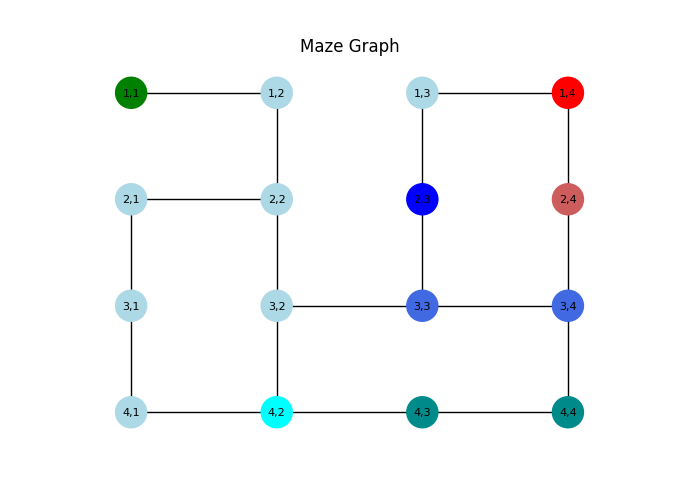
\includegraphics[width=0.5\textwidth]{Cap2/maze_imperfect_exploration.png}
\caption{Exploration of an imperfect maze(graph) by three agents.}
\label{fig_imperfect_maze_exploration}
\end{figure}

This visualization showcases how our algorithm can handle graphs
with cycles, illustrating the adaptability of our approach.

\section{Agent Tree Visualization}
\label{section_method_tree_visualization}

In addition to overall graph exploration,
we developed a method to visualize the individual exploration trees constructed by each agent during the process. These trees represent the paths traversed by the agents and provide insight into the structure of their independent exploration, including how cycles are managed and intervals are assigned to each node.

The Figures \ref{fig_agent_1_tree}, \ref{fig_agent_2_tree} and \ref{fig_agent_3_tree}
show the trees constructed by the 3 agents for the exploration displayed in Figure \ref{fig_imperfect_maze_exploration}.
    
\begin{figure}[H]
\centering
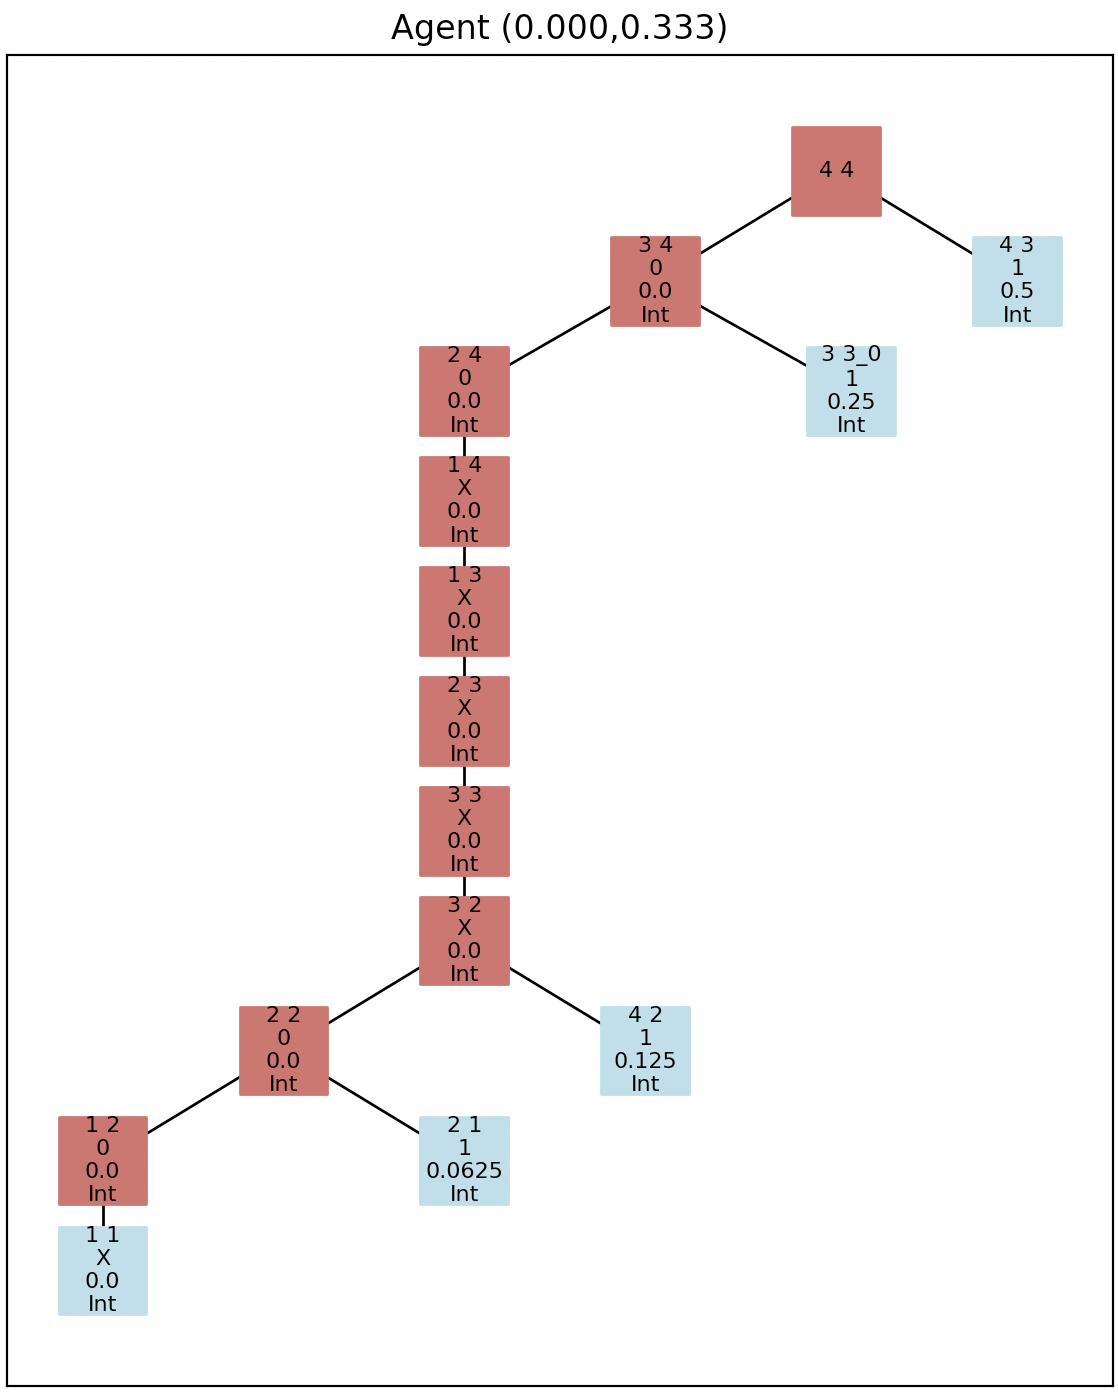
\includegraphics[width=1\textwidth]{Cap2/agent_1.png}
\caption{Trees constructed by agent post-exploration: \textbf{Agent 1}.}
\label{fig_agent_1_tree}
\end{figure}

\begin{figure}[H]
\centering
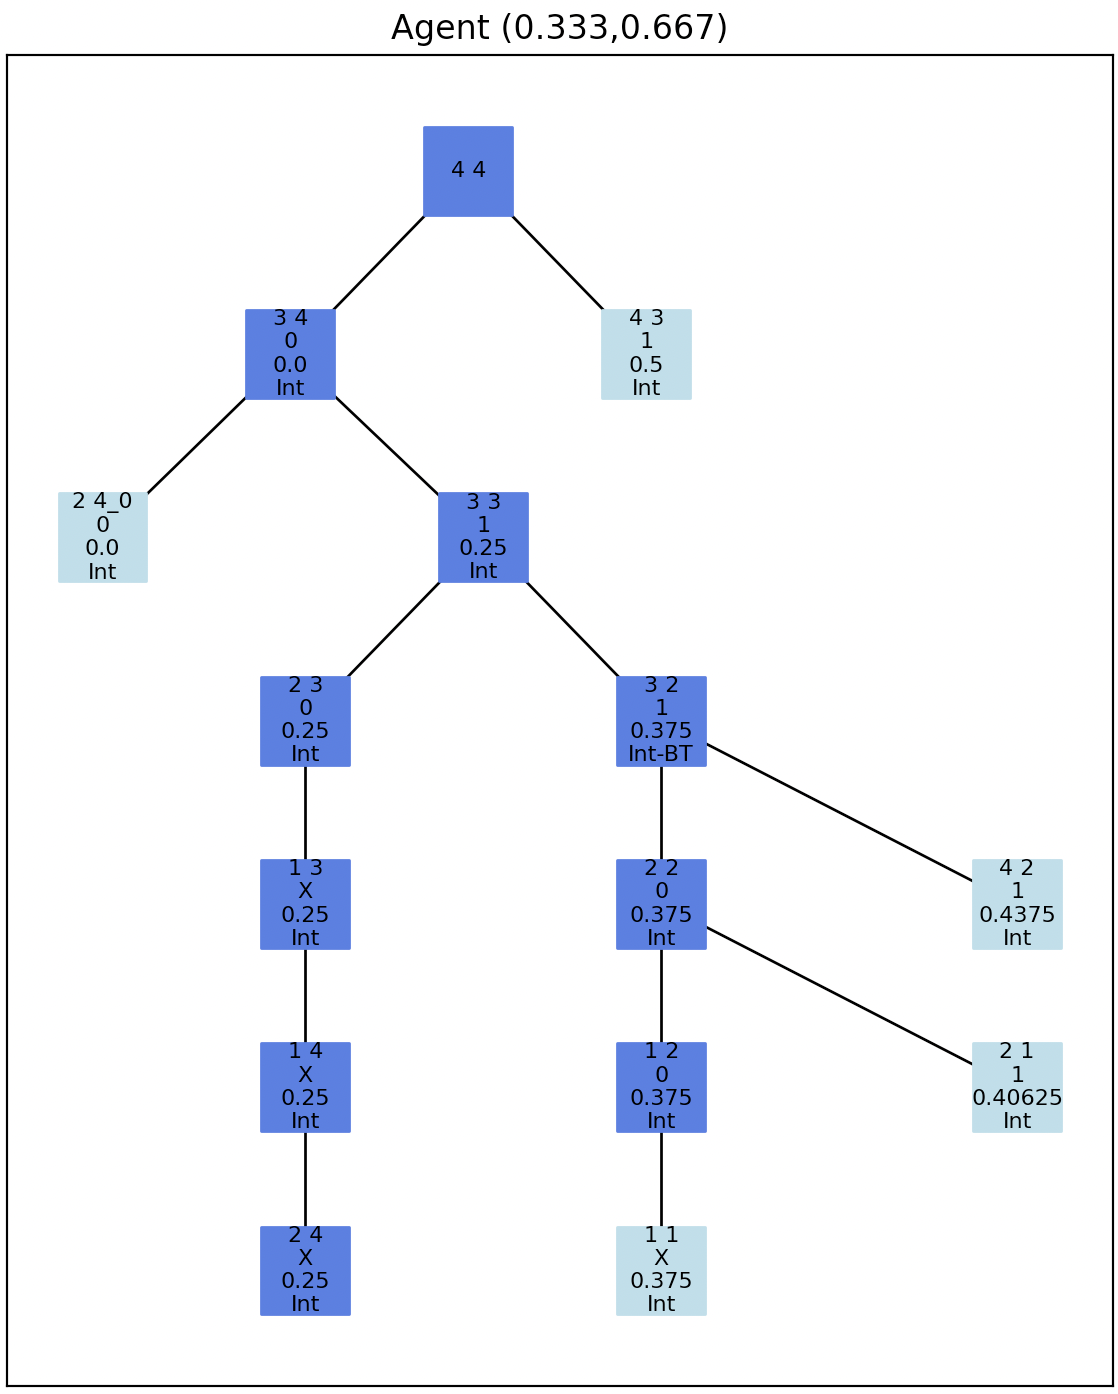
\includegraphics[width=1\textwidth]{Cap2/agent_2.png}
\caption{Trees constructed by agent post-exploration: \textbf{Agent 2}.}
\label{fig_agent_2_tree}
\end{figure}

\begin{figure}[H]
\centering
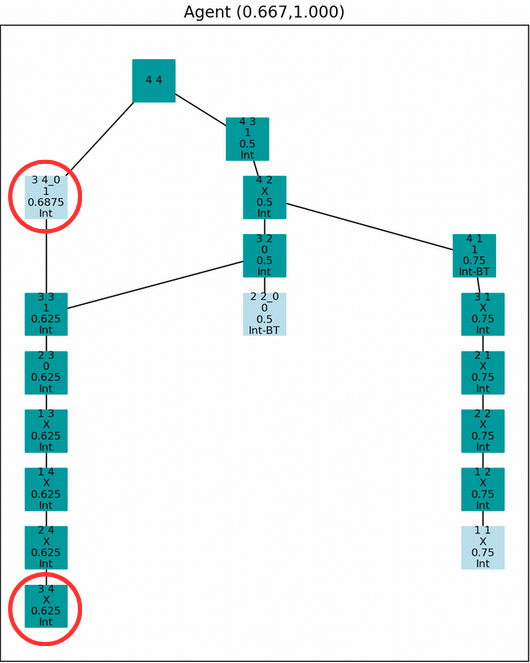
\includegraphics[width=1\textwidth]{Cap2/agent_3.png}
\caption{Trees constructed by agent post-exploration: \textbf{Agent 3}.}
\label{fig_agent_3_tree}
\end{figure}
    

These visualizations illustrate how each agent independently builds its representation of the graph, leading to varied exploration trees. In Figure \ref{fig_agent_3_tree}, the highlighted nodes, $(3, 4)$ and $(3, 4)\_0$, demonstrate how cycles can occur during exploration.

Initially, node $(3, 4)$ was added to the tree when the agent discovered it while exploring the neighbors of node $(4, 4)$, even though it hadn't been visited yet. Later, as the exploration progressed, the agent reached node $(3, 4)$ while checking the neighbors of node $(3, 3)$, revealing a cycle. According to the method outlined in Section \ref{section_method_algorithm}, the original node $(3, 4)$ was removed from the agent's tree to maintain an acyclic structure. For illustration purposes, a copy of the tree was created, and node $(3, 4)$ was re-added with a modified identifier (appending "\_0" to its ID) to visualize this occurrence.

Finally, when node $(3, 4)$ was reached again while exploring the neighbors of node $(2, 4)$, the agent again removed it from its tree and added it as a child of node $(2, 4)$. This step-by-step process clarifies the presence of node $(3, 4)\_0$ in the figure, along with the edges connecting it to nodes $(4, 4)$ and $(3, 3)$, and the edge from node $(2, 4)$ indicating when node $(3, 4)$ was finally explored.